% Michaels Text
\subsection{Support Vector Machine}
\begin{frame}
\frametitle{Analysemethoden}
\framesubtitle{Support Vector Machine}
\begin{itemize}\setlength\parskip{12pt}
\item Versucht Entscheidungsgrenze (Hyperebene) zu finden, die die Distanz der nächsten Datenpunkte jeder Klasse zu ihr maximiert
\item Diese nächsten Datenpunkte sind die \textit{Support Vectors}
\end{itemize}
\begin{figure}
	\centering
	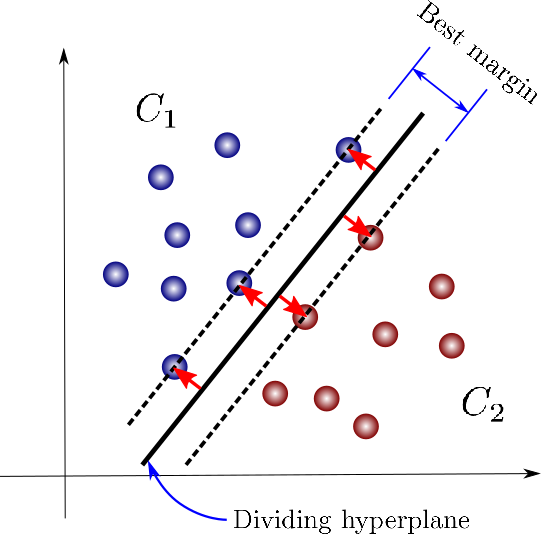
\includegraphics[scale=0.25]{svm.png}\\
	\quelle\url{https://towardsdatascience.com/support-vector-machines-for-classification-fc7c1565e3}
\end{figure}
\end{frame}
%<-------------Folie--------->
\begin{frame}
\frametitle{Analysemethoden}
\framesubtitle{Support Vector Machine}
\begin{itemize}\setlength\parskip{12pt}
	\item Verschiedene Kerne (Funktionen) um dem Separierungsproblem gerecht zu werden
	\item Kerne projizieren nicht-linear separierbare Daten niedrigerer Dimensionen auf linear-separierbare Daten höherer Dimensionen
	\item Vier häufig verwendete Kerne:
	\begin{itemize}
		\item \makebox[3.1cm][l]{Linear} $\langle u, v \rangle$
		\item \makebox[3.1cm][l]{Polynomiell} $(\gamma \langle u, v \rangle + r)^d$
		\item \makebox[3.1cm][l]{Radial} $\exp(-\gamma \| u-v \|^2)$
		\item \makebox[3.1cm][l]{Sigmoidal} $\tanh(\gamma \langle u,v \rangle + r)$
	\end{itemize}
	\item In \texttt{R} mit \texttt{e1071} und in Python mit \texttt{sklearn}
\end{itemize}
\end{frame}
%<-------------Folie--------->
\begin{frame}
\frametitle{Resultate Support Vector Machine}
\begin{center}
Support Vector Machine, \texttt{R}, Wortvorkommen mind. 10 mal,\\
Radialer Kern, Modifizierter CISTEM-Stemmer, Deutsch

\bigskip

\begin{tabular}{|c|c|c|c|c|c|c|c|c|}
\hline
				& D 	& G	& I & S	& Acc.	& Prec. & Recall	& F1\\
\hline
Dominant 		& 14		& 3 			& 8 		& 1 		&       	& 53,8\% 	& 77,8\% 	& 63,6\%\\
Gewissenhaft 	& 0 		& 1 			& 1 		& 0 		& 			& 50,0\% 	& 7,1\% 	& 16,3\%\\
Initiativ 		& 4 		& 10			& 27		& 14		& 			& 57,0\%		& 75,0\% 	& 41,9\%\\
Stetig 			& 0 		& 0 			& 0 		& 3 		& 			& 100\%	   	& 16,7\% 	& 20,9\%\\
\hline
Total 			& 			& 				& 			& 			& 52,33\%	& 63,2\%		& 44,1\%  	& 41,0\%\\
\hline
\end{tabular}
\end{center}
\end{frame}
%<-------------Folie--------->
\begin{frame}
\frametitle{Resultate Support Vector Machine}
\begin{center}
Support Vector Machine, \texttt{Python}, Wortvorkommen mind. 20 mal,\\
Sigmoid Kern, Porter-Stemmer aus \texttt{nltk}, Englisch

\bigskip

\begin{tabular}{|c|c|c|c|c|c|c|c|c|}
\hline
				& D 	& G	& I & S	& Acc.	& Prec. & Recall	& F1\\
\hline
Dominant 		& 14		& 2 			& 9 		& 1 		&       	& 54\%	 	& 78\%	 	& 64\%\\
Gewissenhaft 	& 0 		& 5 			& 4 		& 1 		& 			& 50\%	 	& 36\%	 	& 42\%\\
Initiativ 		& 3 		& 5				& 19		& 13		& 			& 47\%		& 53\%	 	& 50\%\\
Stetig 			& 1 		& 2 			& 4 		& 3 		& 			& 30\%	   	& 17\%	 	& 21\%\\
\hline
Total 			& 			& 				& 			& 			& 47,7\%		& 45\%		& 46\%  	& 44\%\\
\hline
\end{tabular}
\end{center}
\end{frame}
%<-------------Folie--------->
\subsection{Schwierigkeiten}
\begin{frame}
\frametitle{Schwierigkeiten}
\begin{itemize}
	\item Keine eindeutige Klassifikation
	\begin{itemize}
		\item Auch für Menschen nicht eindeutig
		\item Teilweise sehr geringe Unterschiede zwischen den Typen
	\end{itemize}
	\item Stemming nicht unbedingt eindeutig
	\begin{itemize}
		\item Unregelmäßigkeit von Verben im Deutschen
		\item Komposita
	\end{itemize}
	\item Geringe Zahl an Trainingsdaten
	\item Unbalanciertes Studiendesign
	\item Representativität
	\begin{itemize}
		\item Introvertierte Kunden schreiben weniger häufig Reviews
		\item Nur positive Bewertungen lagen vor
	\end{itemize}
\end{itemize}
\end{frame}